\documentclass{article}[18pt]
\ProvidesPackage{format}
%Page setup
\usepackage[utf8]{inputenc}
\usepackage[margin=0.7in]{geometry}
\usepackage{parselines} 
\usepackage[english]{babel}
\usepackage{fancyhdr}
\usepackage{titlesec}
\hyphenpenalty=10000

\pagestyle{fancy}
\fancyhf{}
\rhead{Sam Robbins}
\rfoot{Page \thepage}

%Characters
\usepackage{amsmath}
\usepackage{amssymb}
\usepackage{gensymb}
\newcommand{\R}{\mathbb{R}}

%Diagrams
\usepackage{pgfplots}
\usepackage{graphicx}
\usepackage{tabularx}
\usepackage{relsize}
\pgfplotsset{width=10cm,compat=1.9}
\usepackage{float}

%Length Setting
\titlespacing\section{0pt}{14pt plus 4pt minus 2pt}{0pt plus 2pt minus 2pt}
\newlength\tindent
\setlength{\tindent}{\parindent}
\setlength{\parindent}{0pt}
\renewcommand{\indent}{\hspace*{\tindent}}

%Programming Font
\usepackage{courier}
\usepackage{listings}
\usepackage{pxfonts}

%Lists
\usepackage{enumerate}
\usepackage{enumitem}

% Networks Macro
\usepackage{tikz}


% Commands for files converted using pandoc
\providecommand{\tightlist}{%
	\setlength{\itemsep}{0pt}\setlength{\parskip}{0pt}}
\usepackage{hyperref}

% Get nice commands for floor and ceil
\usepackage{mathtools}
\DeclarePairedDelimiter{\ceil}{\lceil}{\rceil}
\DeclarePairedDelimiter{\floor}{\lfloor}{\rfloor}

% Allow itemize to go up to 20 levels deep (just change the number if you need more you madman)
\usepackage{enumitem}
\setlistdepth{20}
\renewlist{itemize}{itemize}{20}

% initially, use dots for all levels
\setlist[itemize]{label=$\cdot$}

% customize the first 3 levels
\setlist[itemize,1]{label=\textbullet}
\setlist[itemize,2]{label=--}
\setlist[itemize,3]{label=*}

% Definition and Important Stuff
% Important stuff
\usepackage[framemethod=TikZ]{mdframed}

\newcounter{theo}[section]\setcounter{theo}{0}
\renewcommand{\thetheo}{\arabic{section}.\arabic{theo}}
\newenvironment{important}[1][]{%
	\refstepcounter{theo}%
	\ifstrempty{#1}%
	{\mdfsetup{%
			frametitle={%
				\tikz[baseline=(current bounding box.east),outer sep=0pt]
				\node[anchor=east,rectangle,fill=red!50]
				{\strut Important};}}
	}%
	{\mdfsetup{%
			frametitle={%
				\tikz[baseline=(current bounding box.east),outer sep=0pt]
				\node[anchor=east,rectangle,fill=red!50]
				{\strut Important:~#1};}}%
	}%
	\mdfsetup{innertopmargin=10pt,linecolor=red!50,%
		linewidth=2pt,topline=true,%
		frametitleaboveskip=\dimexpr-\ht\strutbox\relax
	}
	\begin{mdframed}[]\relax%
		\centering
		}{\end{mdframed}}



\newcounter{lem}[section]\setcounter{lem}{0}
\renewcommand{\thelem}{\arabic{section}.\arabic{lem}}
\newenvironment{defin}[1][]{%
	\refstepcounter{lem}%
	\ifstrempty{#1}%
	{\mdfsetup{%
			frametitle={%
				\tikz[baseline=(current bounding box.east),outer sep=0pt]
				\node[anchor=east,rectangle,fill=blue!20]
				{\strut Definition};}}
	}%
	{\mdfsetup{%
			frametitle={%
				\tikz[baseline=(current bounding box.east),outer sep=0pt]
				\node[anchor=east,rectangle,fill=blue!20]
				{\strut Definition:~#1};}}%
	}%
	\mdfsetup{innertopmargin=10pt,linecolor=blue!20,%
		linewidth=2pt,topline=true,%
		frametitleaboveskip=\dimexpr-\ht\strutbox\relax
	}
	\begin{mdframed}[]\relax%
		\centering
		}{\end{mdframed}}
\lhead{MCS - Logic and Discrete Structures}
\usepackage{soul}


\begin{document}
\begin{center}
\underline{\huge Resolution for Propositional Logic}
\end{center}
\section{Resolution}
Recall the rule of inference known as resolution:
\begin{center}
	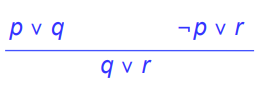
\includegraphics[scale=0.7]{resolution}
\end{center}
\begin{itemize}
	\item Forms the basis of the proof system for propositional logic known as \textbf{resolution}
\end{itemize}
However, the basic rule of resolution is a more general one than that above
\begin{center}
	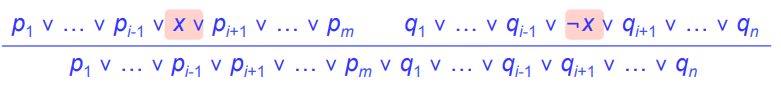
\includegraphics[scale=0.7]{basic_resolution}
\end{center}
\begin{itemize}
	\item The ps and qs are literals - that is, variables or negated variables (not necessarily distinct)
	\item This is the \textbf{only} rule of resolution
\end{itemize}
This idea can also be implied with just $x$ and $\lnot x$ the empty set can be inferred as there is a contradiction.
\section{The proof system Resolution}
\begin{itemize}
	\item Natural deduction proves theorems starting from scratch, whereas resolution takes a given formula and works with it in order to decide whether it is a theorem or not
	\item In the proof system resolution, we proceed as follows
	\begin{itemize}
		\item We are given a propositional formula $\varphi$
		\item We take $\lnot\varphi$ and write it in cnf as $C_1\land C_2\land...\land C_m$
		\item We start with the clauses $C_1,C_2,...,C_m$
		\item We continually apply the resolution rule of inference to infer new clauses
		\begin{itemize}
			\item If we infer the empty clause $\varnothing$, then we halt and output that $\varphi$ is a theorem
			\item If we get to the point where we have not inferred the empty clause and we cannot infer any new clauses then we halt and output that $\varphi$ is not a theorem
		\end{itemize}
	\end{itemize}
	\item We have one minor remark
	\begin{itemize}
		\item When resolving, we are also allowed to delete the repeated literals in any clause
	\end{itemize}
	\item Resolution is both sound and complete
	\begin{itemize}
		\item if Resolution announces that $\varphi$ is a theorem then $\varphi$ is a tautology
		\item if $\varphi$ is a tautology then Resolution announces that $\varphi$ is a theorem
	\end{itemize}
\end{itemize}
\section{Resolution in action}
Consider the propositional formula $\varphi$
\begin{center}
	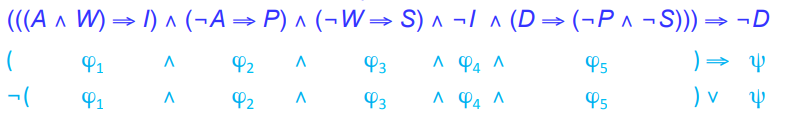
\includegraphics[scale=0.7]{phi}
\end{center}
So $\lnot \varphi$ is
\begin{center}
	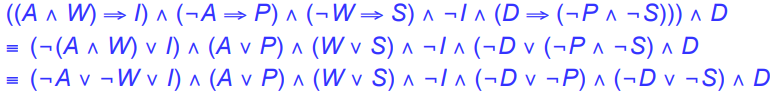
\includegraphics[scale=0.7]{notphi}
\end{center}
So, the set of clauses to which we apply resolution is:
$$\lnot A \lor \lnot W \lor I \qquad A \lor P \qquad W \lor S \qquad \lnot I\qquad \lnot D \lor \lnot P \qquad \lnot D \lor \lnot S \qquad D $$
\section{Resolution in action}
So, we have our set of clauses
$$\lnot A \lor \lnot W \lor I \qquad A \lor P \qquad W \lor S \qquad \lnot I\qquad \lnot D \lor \lnot P \qquad \lnot D \lor \lnot S \qquad D $$
Now we start resolving
\begin{itemize}
	\item $\lnot A\lor \lnot W$ ($\lnot A\lor \lnot W\lor I$ and $\lnot I$)
	\item $P\lor \lnot W$ ($\lnot A \lor \lnot W$ and $A\lor P$)
	\item  $P\lor S$ ($P\lor \lnot W$ and $W\lor S$)
	\item $\lnot D \lor S$ ($P\lor S$ and $\lnot D\lor \lnot P$)
	\item $\lnot D\lor \lnot D$ ($\lnot D \lor S$ and $\lnot D\lor \lnot S$)
	\item $\lnot D$
	\item $\varnothing$ 
\end{itemize}
So $\varphi$ is a theorem, and so a tautology
\section{Resolution in action}
Let $\varphi$ be the formula $((p\lor q)\land (\lnot p\lor \lnot q)\lor (r\Rightarrow (p\land q)))\Rightarrow r$\\
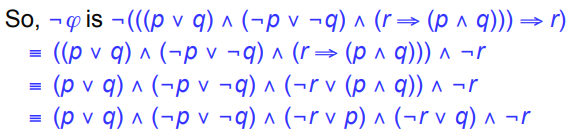
\includegraphics[scale=0.7]{action}\\
Hence, the set of clauses to which we apply resolution is
$$p\lor q \qquad \lnot p\lor \lnot q \qquad \lnot r\lor p \qquad \lnot r\lor q \qquad \lnot r$$
Now we start resolving
\begin{itemize}
	\item \st{$q\lor\lnot q$} - we can ignore this as it will never yield a new clause
	\item \st{$p\lor\lnot p$} - we can ignore this as it will never yield a new clause
	\item $\lnot q \lor \lnot r$
	\item $\lnot p\lor \lnot r$
	\item \st{$p\lor\lnot r$} - we have this phrase already
	\item \st{$\lnot r\lor \lnot r$} - i.e. $\lnot r$ and we have this clause already 
	\item \st{$\lnot q \lor \lnot r$} - we have this clause already
	\item \st{$\lnot r\lor \lnot r$} - i.e. $\lnot r$ and we have this clause already 
	\item No new clauses can be inferred 
\end{itemize}
If you have n non negated clauses and l negated clauses, then the number of new clauses is $n\times l$
\section{Is Resolution the silver bullet}
\begin{itemize}
	\item Resolution works by taking the negation of a formula $\varphi$ we wish to prove true and showing that this negation $\lnot \varphi$ is unsatisfiable (in essence)
	\item One might be inclined to think (from our examples) that resolution will always give a "quick" answer as to whether a formula is a tautology or not
	\item However this is not the case, for the worst case resolution involves an exponential number of applications
\end{itemize}
\section{Satisfiability vs tautologies}
\begin{itemize}
	\item SAT-solvers check whether or not a given formula of propositional logic is satisfiable, whereas proof systems, such as resolution, aim to prove theorems
	\item To some extent, these two tasks are different sides of the same coin
	\item Let $\varphi$ be some propositional formula
	\begin{itemize}
		\item If $\varphi$ is satisfiable
		\begin{itemize}
			\item Then there exists a truth assignment making $\varphi$ true
			\item Therefore $\lnot \varphi$ is not a tautology
		\end{itemize}
		\item Conversely, if $\lnot \varphi$ is not a tautology
		\begin{itemize}
			\item Then there exists some truth assignment making $\lnot\varphi$ false
			\item So $\varphi$ is satisfiable
		\end{itemize}
	\end{itemize}
	\item So, $\varphi$ is satisfiable if, and only if $\lnot \varphi$ is not a tautology
	\begin{itemize}
		\item This leads to strong links between SAT-solving and automated theorem proving
	\end{itemize} 
\end{itemize}

\end{document}